%  Copyright 2020-2026 Robert Bosch GmbH
%
%  Licensed under the Apache License, Version 2.0 (the "License");
%  you may not use this file except in compliance with the License.
%  You may obtain a copy of the License at
%
%      http://www.apache.org/licenses/LICENSE-2.0
%
%  Unless required by applicable law or agreed to in writing, software
%  distributed under the License is distributed on an "AS IS" BASIS,
%  WITHOUT WARRANTIES OR CONDITIONS OF ANY KIND, either express or implied.
%  See the License for the specific language governing permissions and
%  limitations under the License.

\section{Configuration}
Before using Roo Code, you must configure an AI Language Model.
You can choose between AI Providers models, local models (via Ollama) or
GitHub Copilot.

Now, get started by selecting your preferred model provider as shown below:

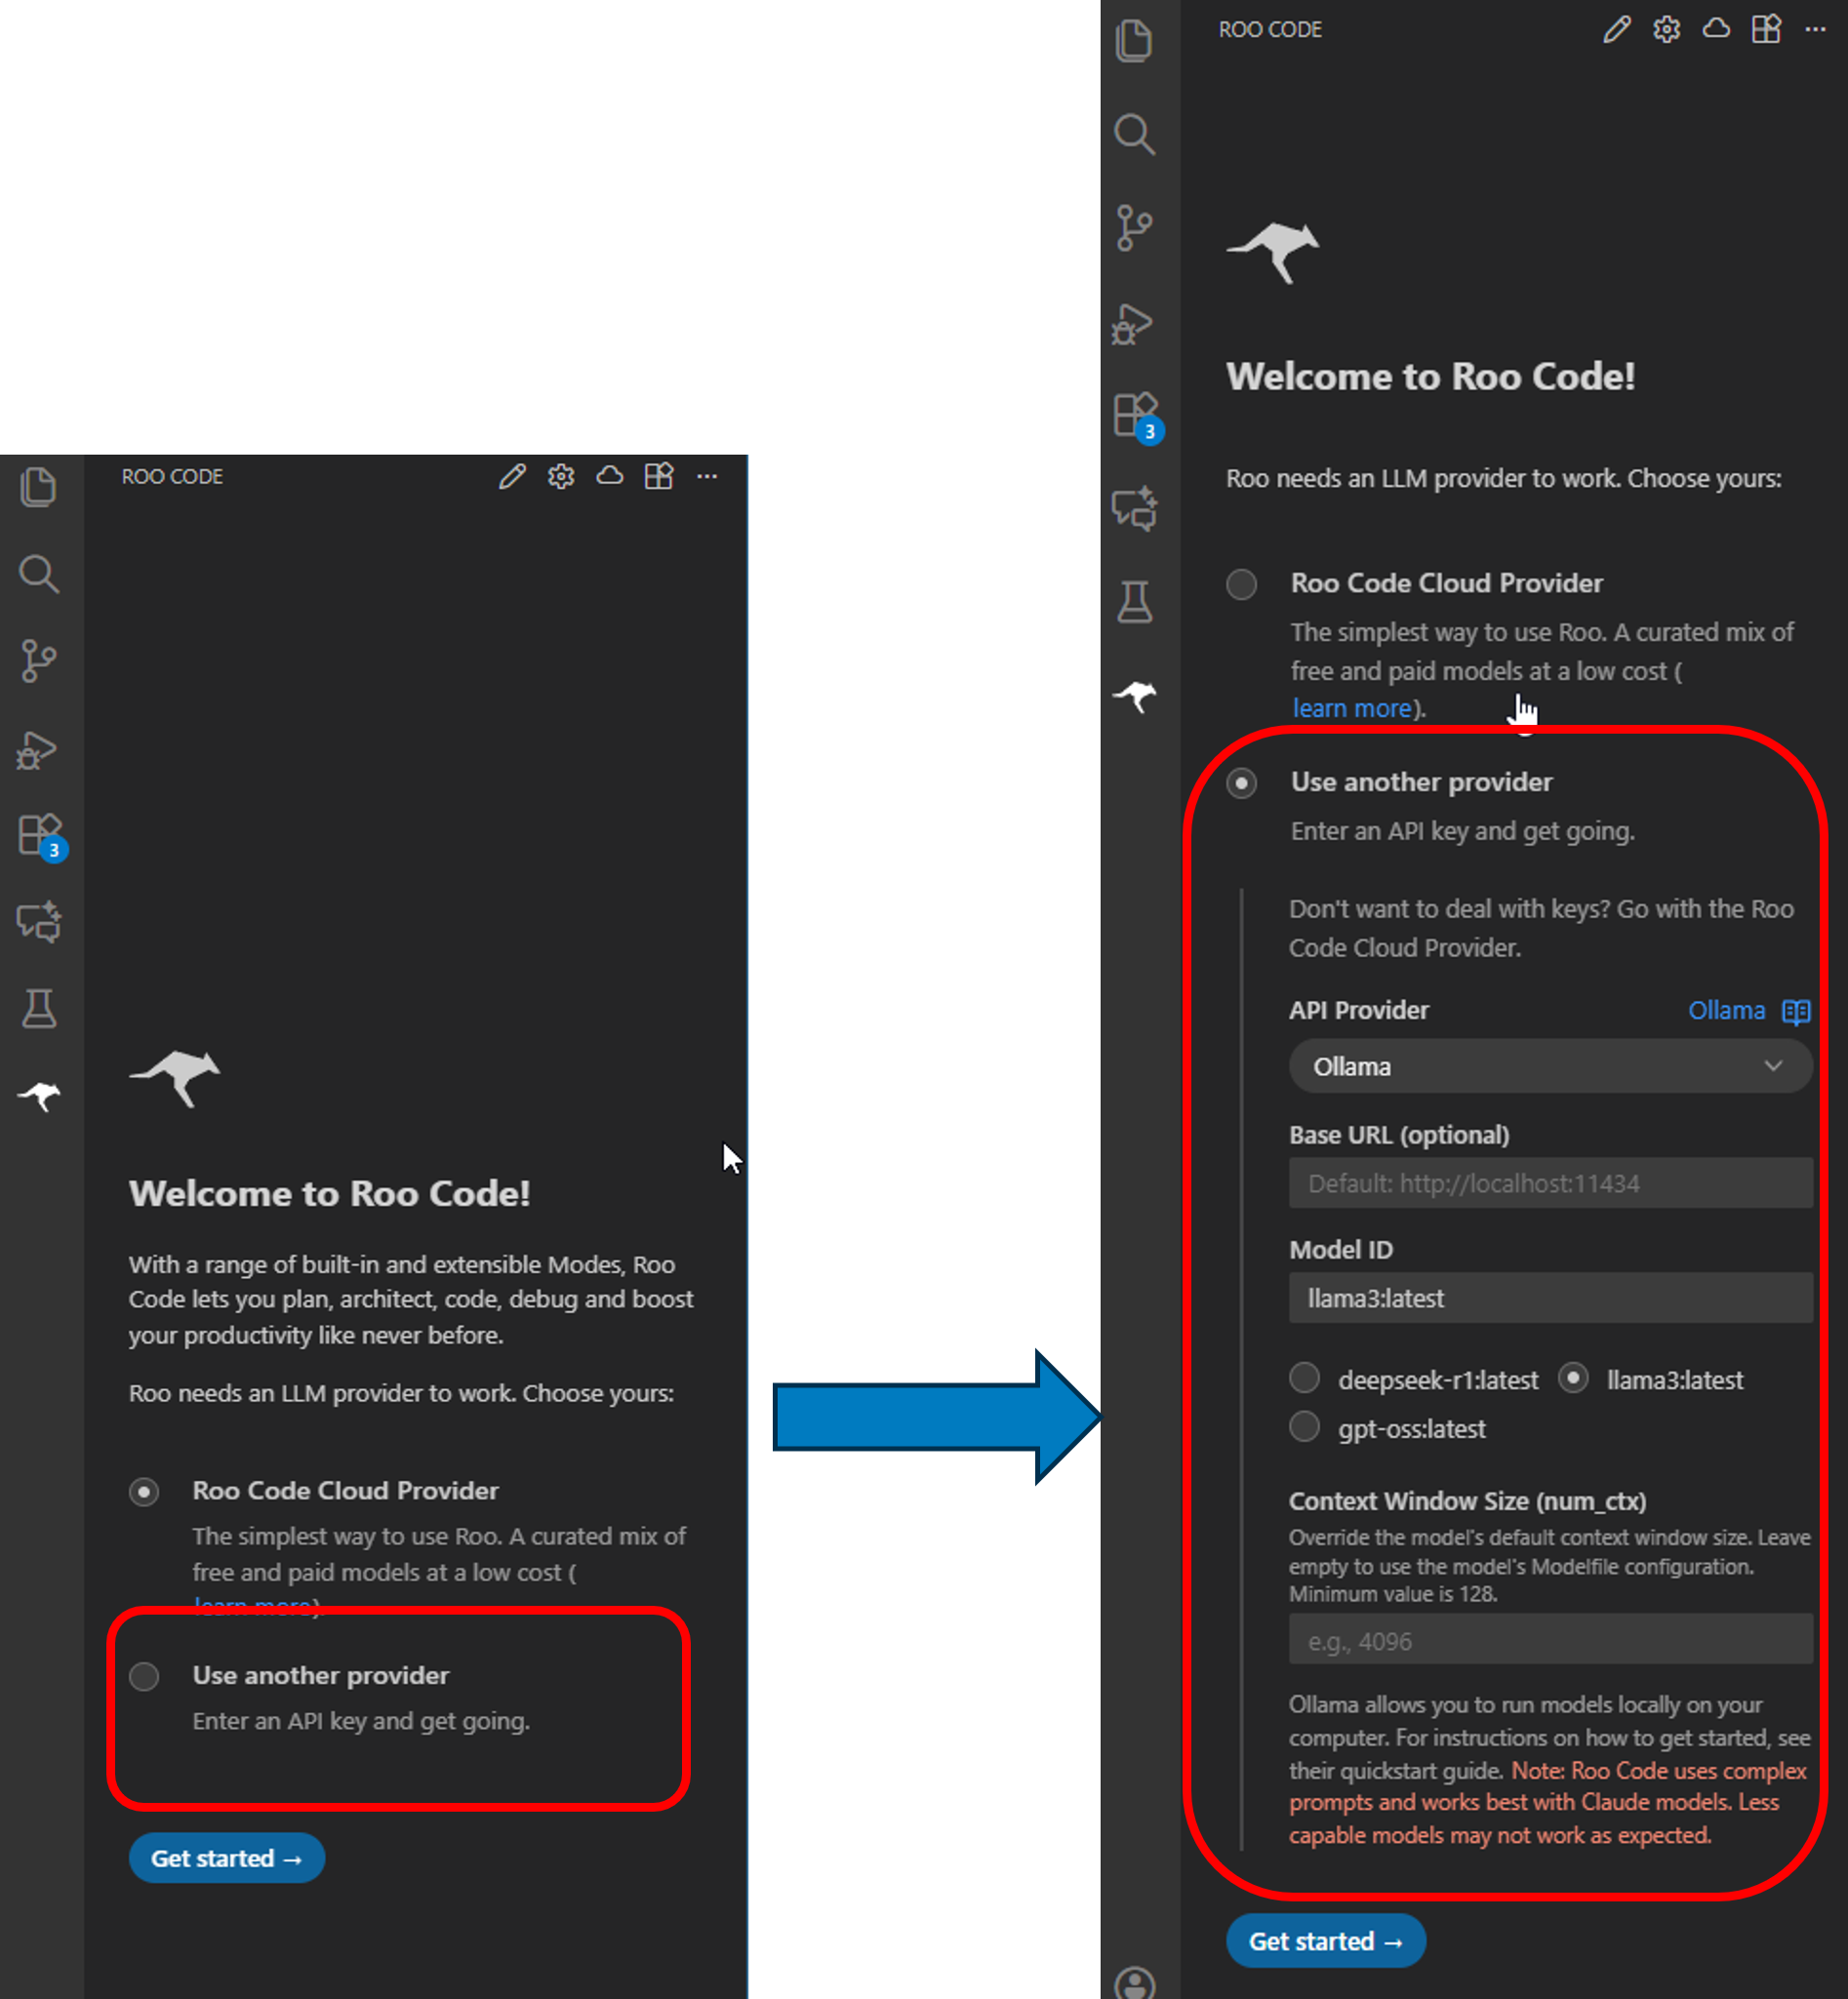
\includegraphics{./include/graphics/roocode/RooCodeUseLLMProviders.png}

\subsection{API Provider Configuration}
\begin{boxhint}{Pre-condition}
You must obtain an API Key from a provider.
List of supported AI service providers:
\begin{itemize}
   \item OpenAI
   \item Google Gemini
   \item Anthropic
   \item \dots
\end{itemize}
\end{boxhint}

\begin{enumerate}
   \item Open \textbf{VSCodium For RobotFramework}.
   \item Click the \textbf{Roo Code icon} in the Activity Bar.
   \item Select \textbf{Use another provider} option at Welcome screen of extension (First time use).

         Or click the \textbf{Settings (gear icon)} at the top of the Roo Code panel (Already configured).
   \item Select your provider (e.g., \textbf{Anthropic} for Claude 3.5 Sonnet).
   \item Enter your \textbf{API Key}.
   \item Choose the specific model (e.g., \texttt{claude-3-5-sonnet-20241022}).
   \item Click \textbf{Done}.
\end{enumerate}

Refer to the image below for an example of using \textbf{Google Gemini} as
the API provider:

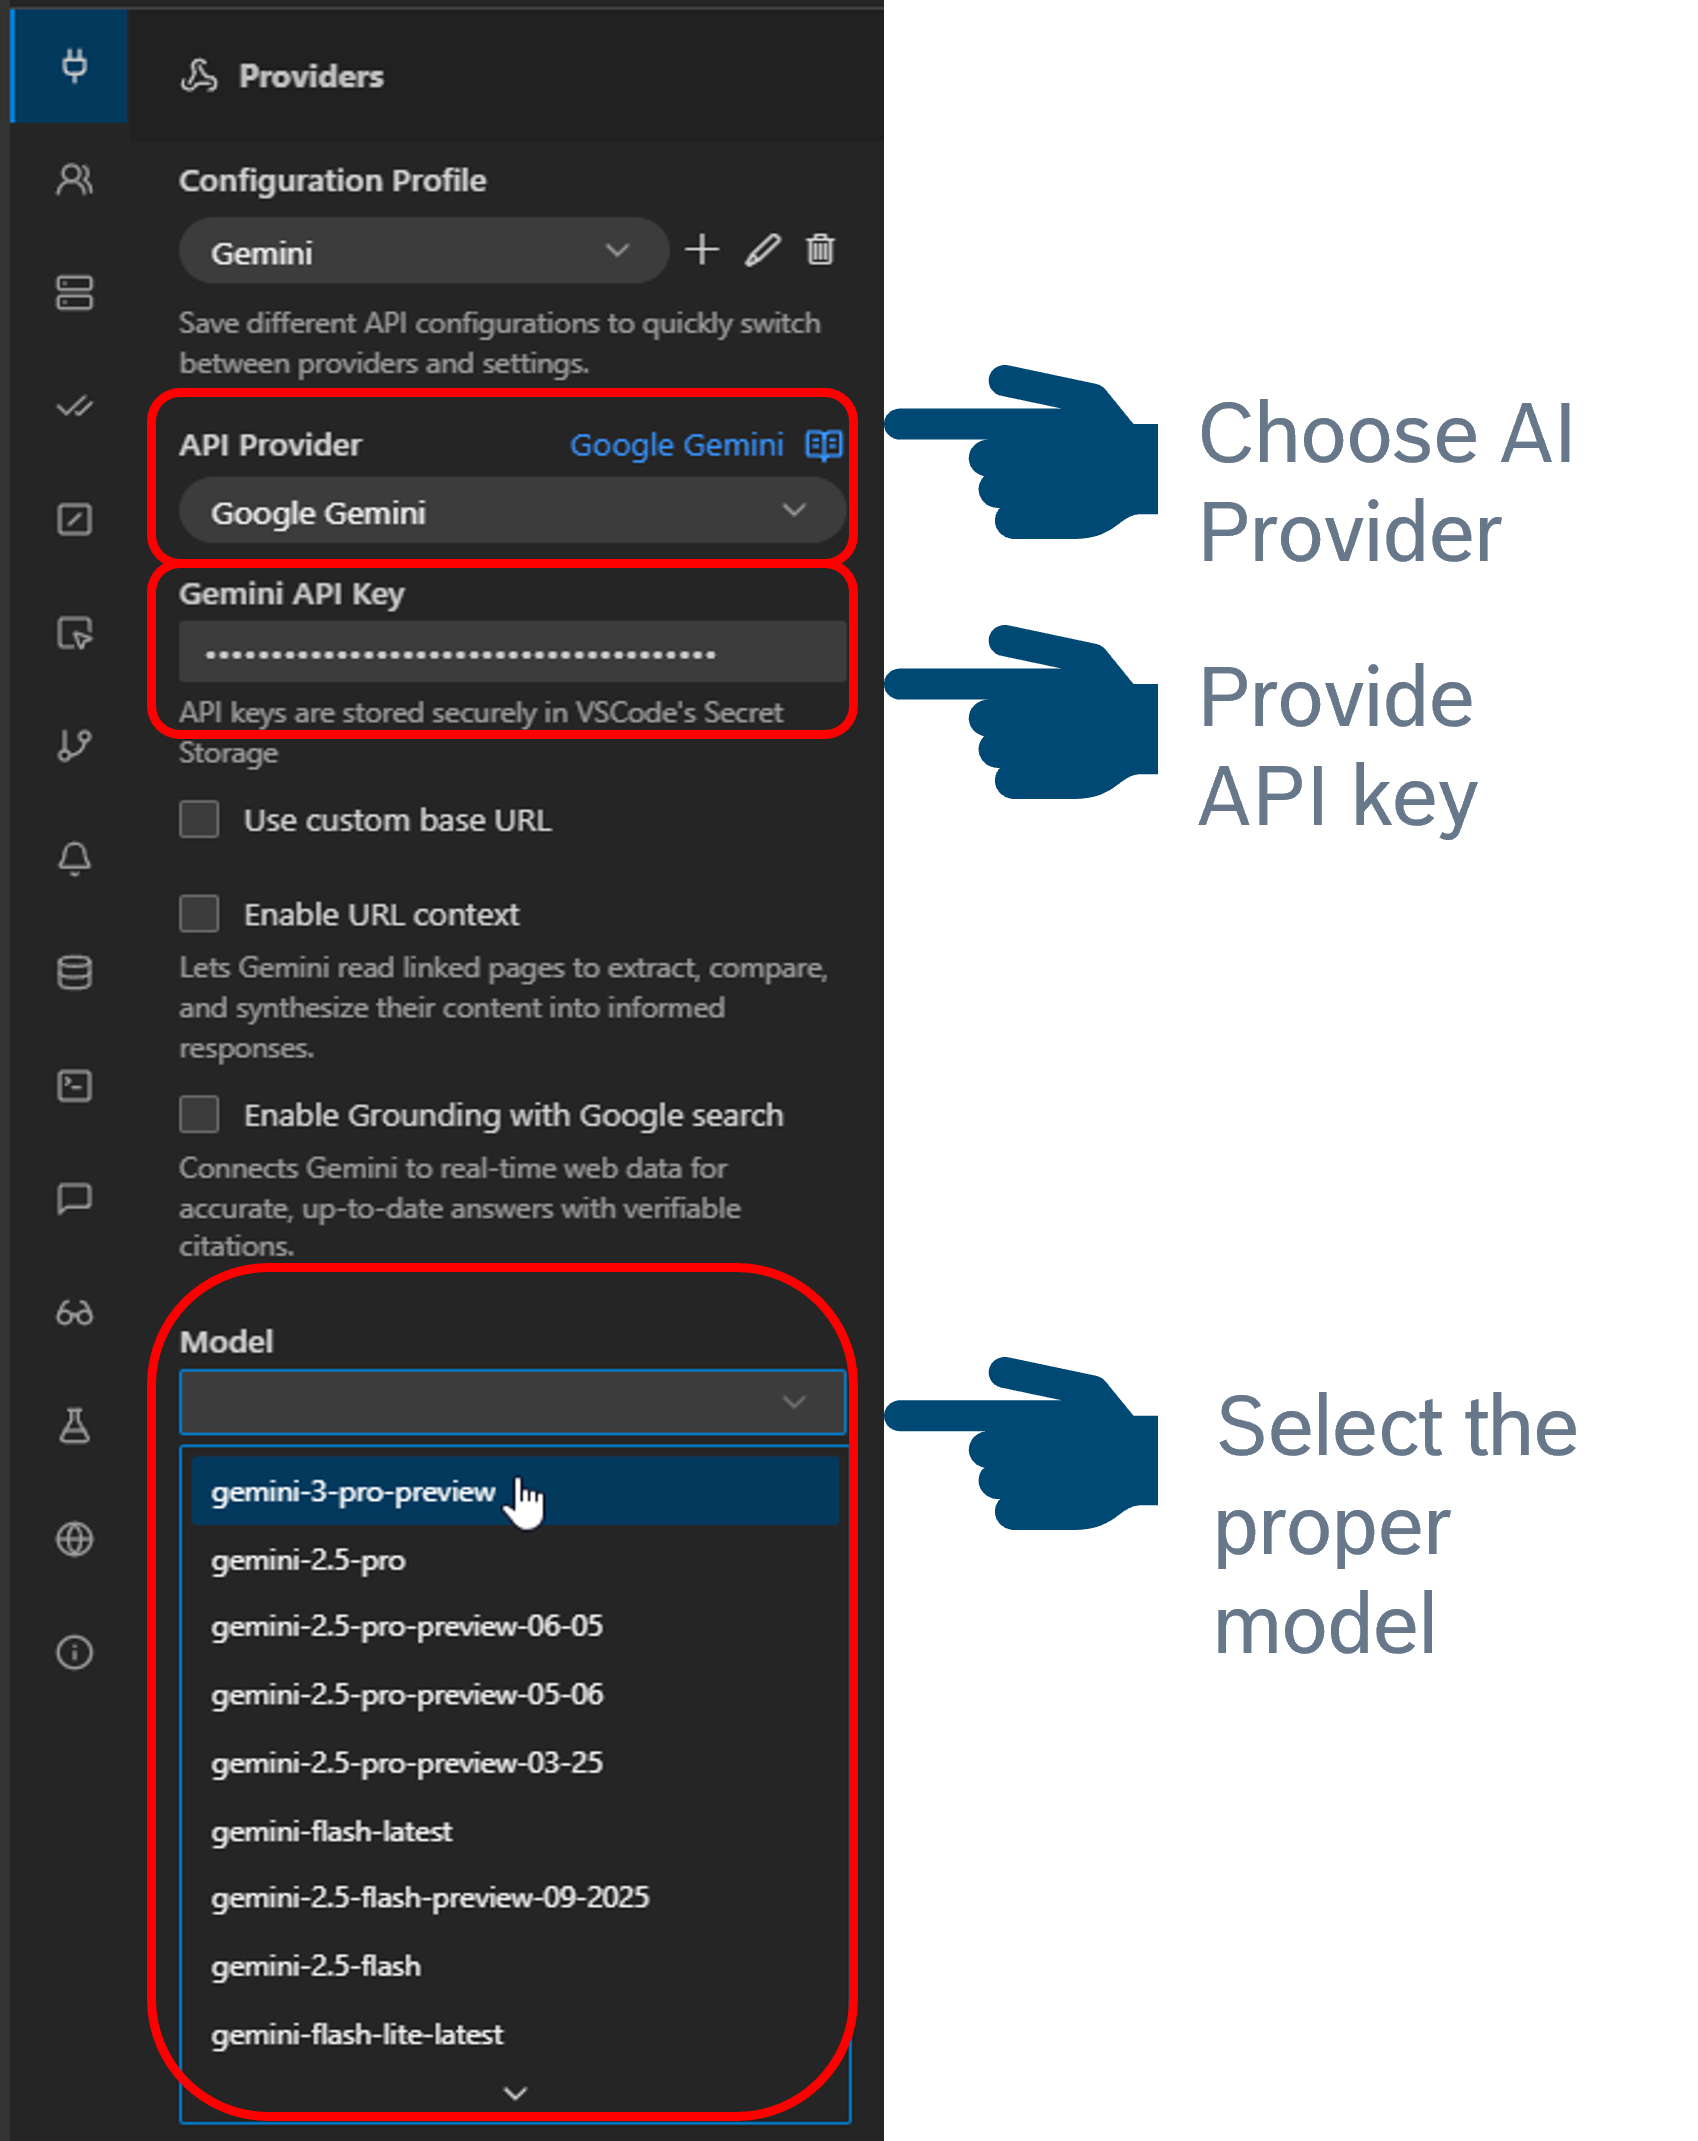
\includegraphics{./include/graphics/roocode/AIProviders.png}

\subsection{Local Model Setup (Ollama)}
For maximum privacy, you can run models locally.
\begin{boxhint}{System Requirement}
Running local models requires significant RAM/GPU resources.
\end{boxhint}

\begin{boxhint}{Pre-condition}
   You need to have Ollama installed and a local model downloaded.
   \begin{itemize}
      \item Download and install Ollama from
         \href{https://ollama.com/download}{Download Ollama}
      \item Use Ollama CLI to pull a coding model:
         \texttt{ollama pull deepseek-v3.1} or \texttt{ollama pull qwen3-coder}.
         You can find other models provided by Ollama at
         \href{https://ollama.com/library}{Ollama Library}.
      \item Ensure Ollama and pulled models are running locally on your machine.

            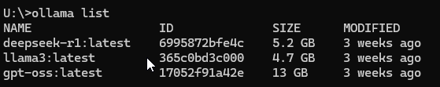
\includegraphics{./include/graphics/roocode/OllamaModels.png}
   \end{itemize}

\end{boxhint}

Steps to configure Roo Code with \textbf{Ollama}:
\begin{enumerate}
   \item Open \textbf{VSCodium For RobotFramework}.
   \item Click the \textbf{Roo Code icon} in the Activity Bar.
   \item Select \textbf{Use another provider} option at Welcome screen of extension (First time use).

         Or click the \textbf{Settings (gear icon)} at the top of the Roo Code panel (Already configured).
   \item In the \textbf{API Provider} option, select \textbf{Ollama}
      as the provider.
   \item Ensure the Base URL is set (usually \texttt{http://localhost:11434}).
   \item Choose the local model you pulled earlier.
   \item Click \textbf{Done}.
\end{enumerate}

Refer to the image below for guidance:

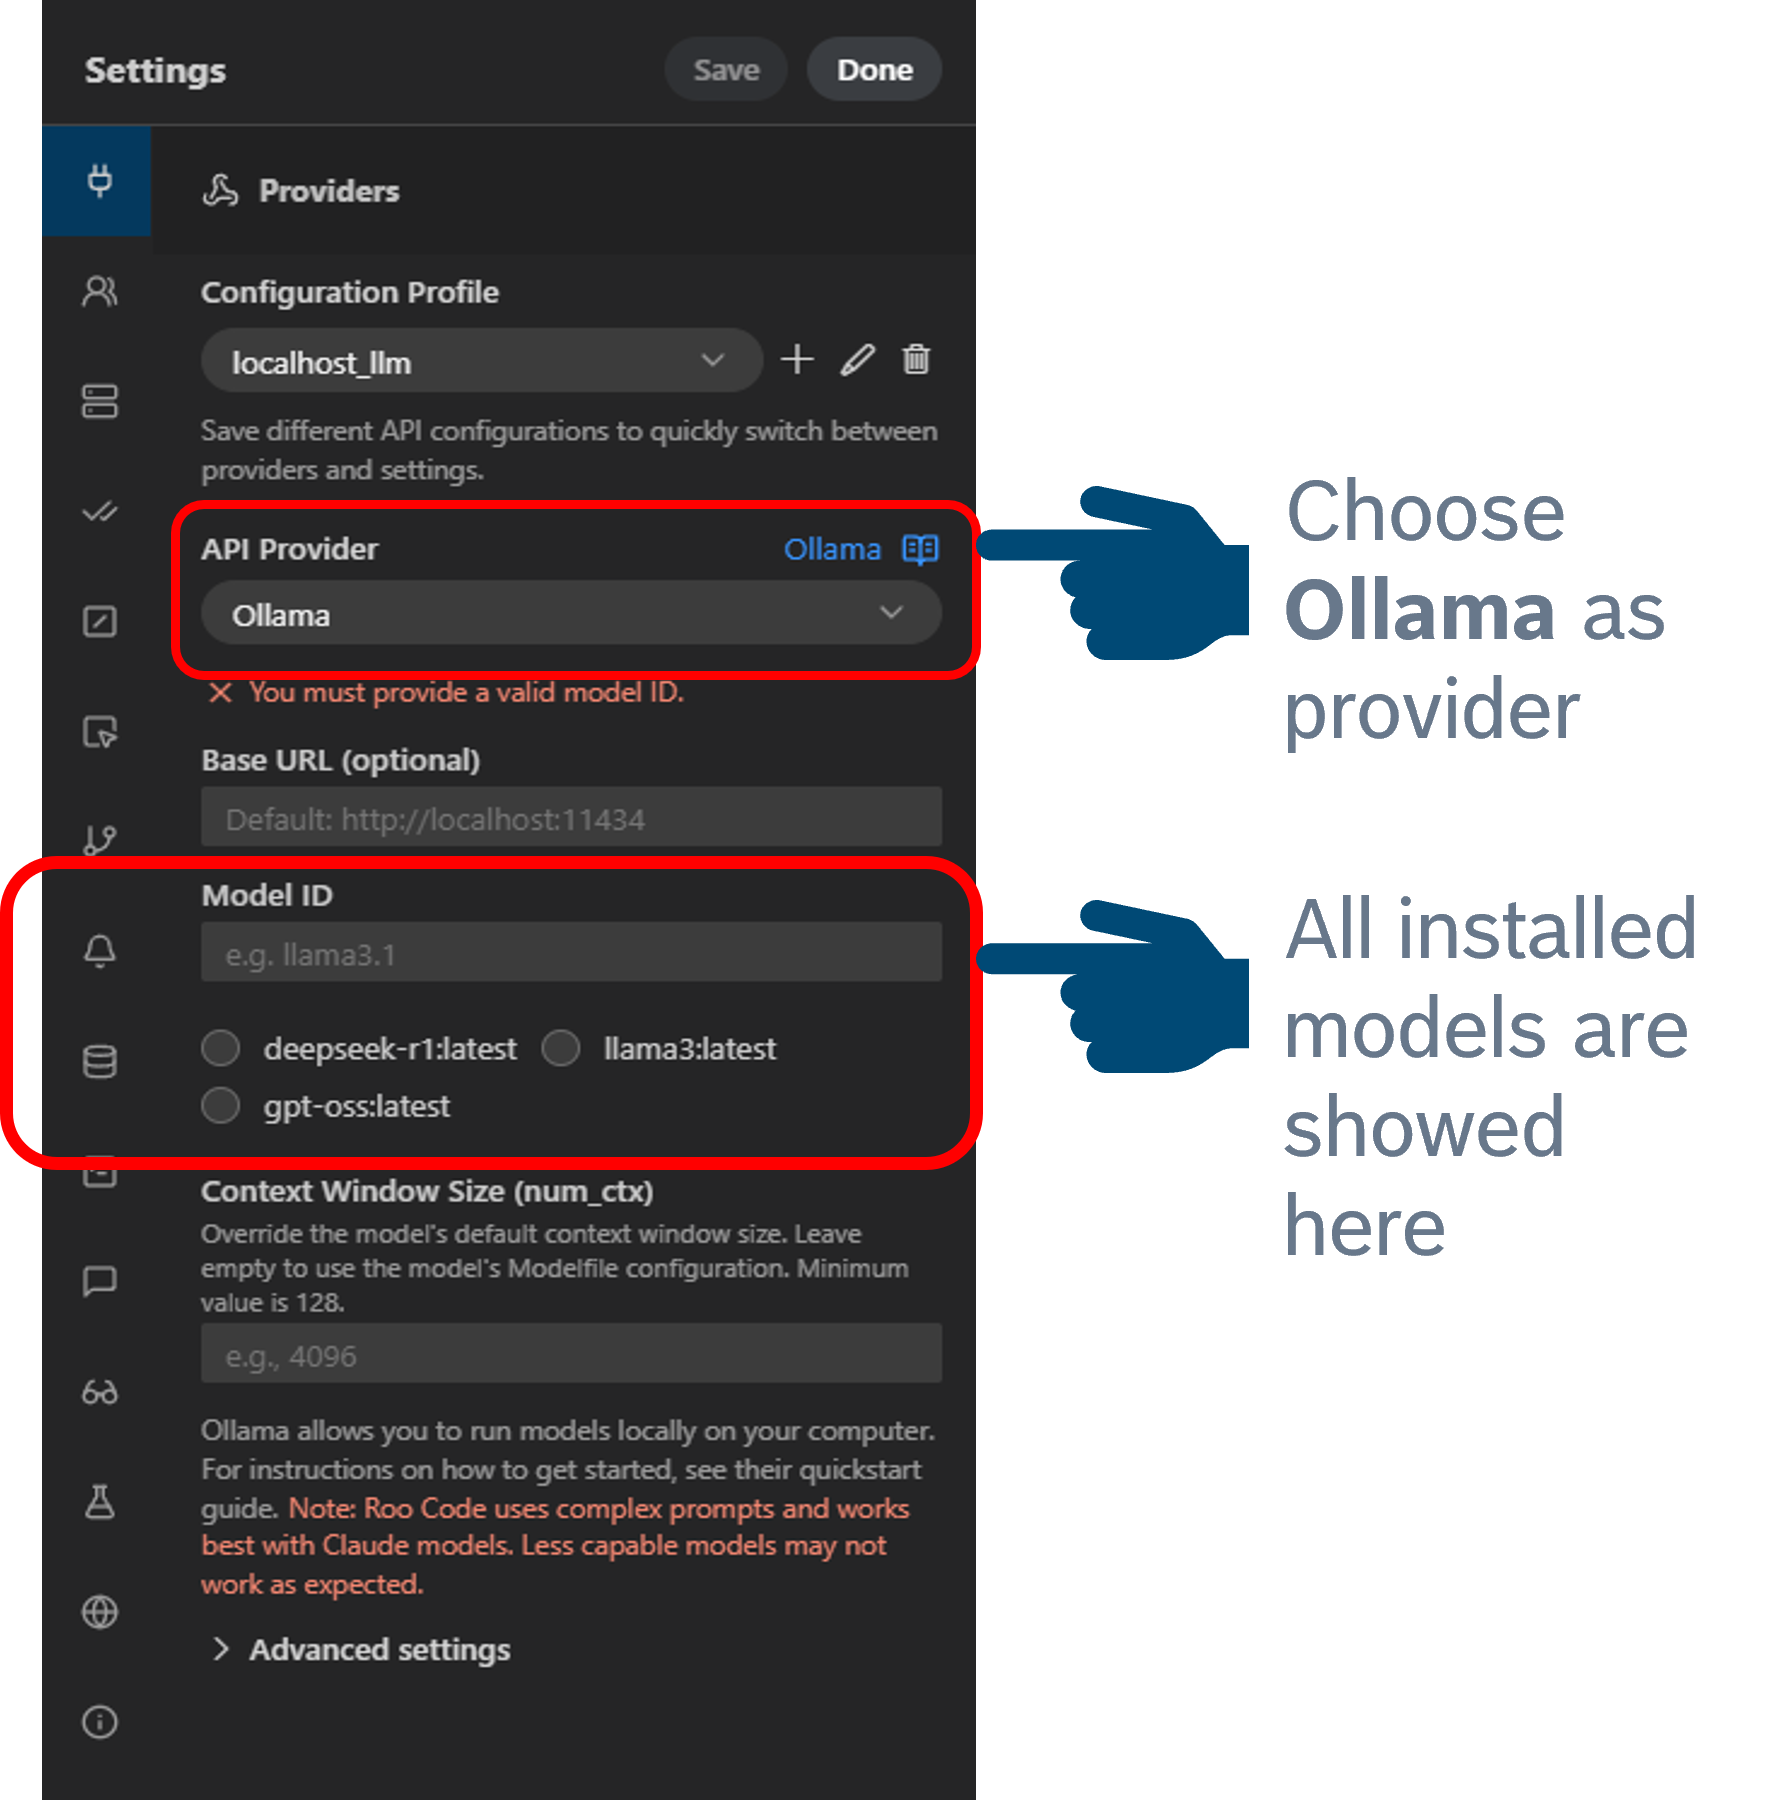
\includegraphics{./include/graphics/roocode/OllamaProvider.png}

\subsection{GitHub Copilot Integration}
Roo Code can leverage your existing GitHub Copilot subscription as
an API source.

\begin{boxhint}{Pre-condition}
Ensure the \textbf{GitHub Copilot} Extensions are installed and you are signed
in with your GitHub account.

Please refer to the chapter \hyperref[chap:copilot]{GitHub Copilot Extension}
for detailed installation and sign-in instructions.

\end{boxhint}

Steps to configure Roo Code with \textbf{GitHub}:
\begin{enumerate}
   \item Open \textbf{VSCodium For RobotFramework}.
   \item Click the \textbf{Roo Code icon} in the Activity Bar.
   \item Select \textbf{Use another provider} option at Welcome screen of extension (First time use).

         Or click the \textbf{Settings (gear icon)} at the top of the Roo Code panel (Already configured).
   \item In the \textbf{API Provider} option, select \textbf{VS Code LM API}
      as the provider.
   \item Choose the available model within the dropdown menu.
   \item Click \textbf{Done}.
\end{enumerate}

Refer to the image below for guidance:

\includegraphics{./include/graphics/roocode/GitHubCopilotLLM.png}
